\documentclass[a4paper, 12pt]{extarticle}
\usepackage[dvipsnames]{xcolor}
\usepackage[top=70pt,bottom=70pt,left=48pt,right=46pt]{geometry}
\definecolor{header}{RGB}{92,184,92}
\definecolor{defenition}{RGB}{217,83,79}
\definecolor{main_title}{RGB}{66,139,202}
\definecolor{sub_header}{RGB}{91,192,222}
\usepackage[english, russian]{babel}
\usepackage[utf8]{inputenc}
\usepackage{amsmath}
\usepackage{listings}
\usepackage{graphicx}
\usepackage{amsmath}
\title{\textcolor{main_title}{Вибрационный магнитометр}}
\author{Шмаков Владимир Евгеньевич - ФФКЭ гр. Б04-105}






\begin{document}
\maketitle



\section*{\textcolor{header}{Цель работы}}

\begin{enumerate}
    \item Ознакомиться с принципом работы вибрационного магнитометра
    \item Ознакомиться с некоторыми методами обработки аналоговых сигналов, получаемых в физических экспериментах 
\end{enumerate}


\section*{\textcolor{header}{Методика}}
\subsection*{\textcolor{sub_header}{Оборудование}}

\begin{itemize}
    \item Вибропреобразователь(используется широкополосный динамик)
    \item Узкополосный фильтр
    \item Катушки малой индуктивности(используемые для приёма сигнала)
    \item Катушки большой индуктивности, используемые в качестве электромагнита
    \item Генератор сигналов 
    \item Синхронный детектор
\end{itemize}

\subsection*{\textcolor{sub_header}{Экспериментальная установка}}

\begin{figure}[htbp]
    \centering
    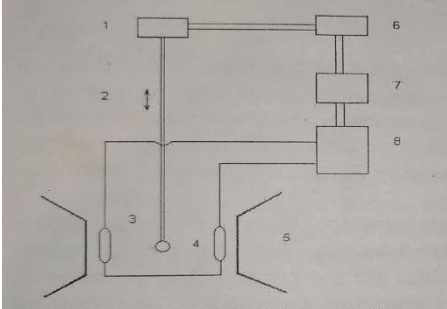
\includegraphics[width = 0.4\textwidth]{ustanovka.png}
    \caption{Схема экпериментальной устновки}
    \label{fig:setup}
\end{figure}

Схема экспериментальной установки изображена на рисунке \ref{fig:setup}.
Шток(2) приводится в колебания посредством динамика (1). Образец (3) находится в поле, создаваемом электромагнитом (5). В результате колебаний на приёмных катушках (4) наводится ЭДС индукции. Полученный с катушек сигнал обрабатывается и усиливается(про алгоритм обработки будет расказанно ниже). Амплитуда обработанного сигнала пропорциональна величине магнитного момента образца.

\subsection*{\textcolor{sub_header}{Методика увеличения динамического диапазона}}




Пусть $S(t)$ - полезный сигнал. $n(t)$ - шумы установки. То есть на вход системы поступает сигнал $S(t) + n(t)$. Входной сигнал амплитудно модулируется высокочастотной синусоидой(смотрите рисунок \ref{fig:input_signals}).

\begin{figure}[htbp]
    \centering
    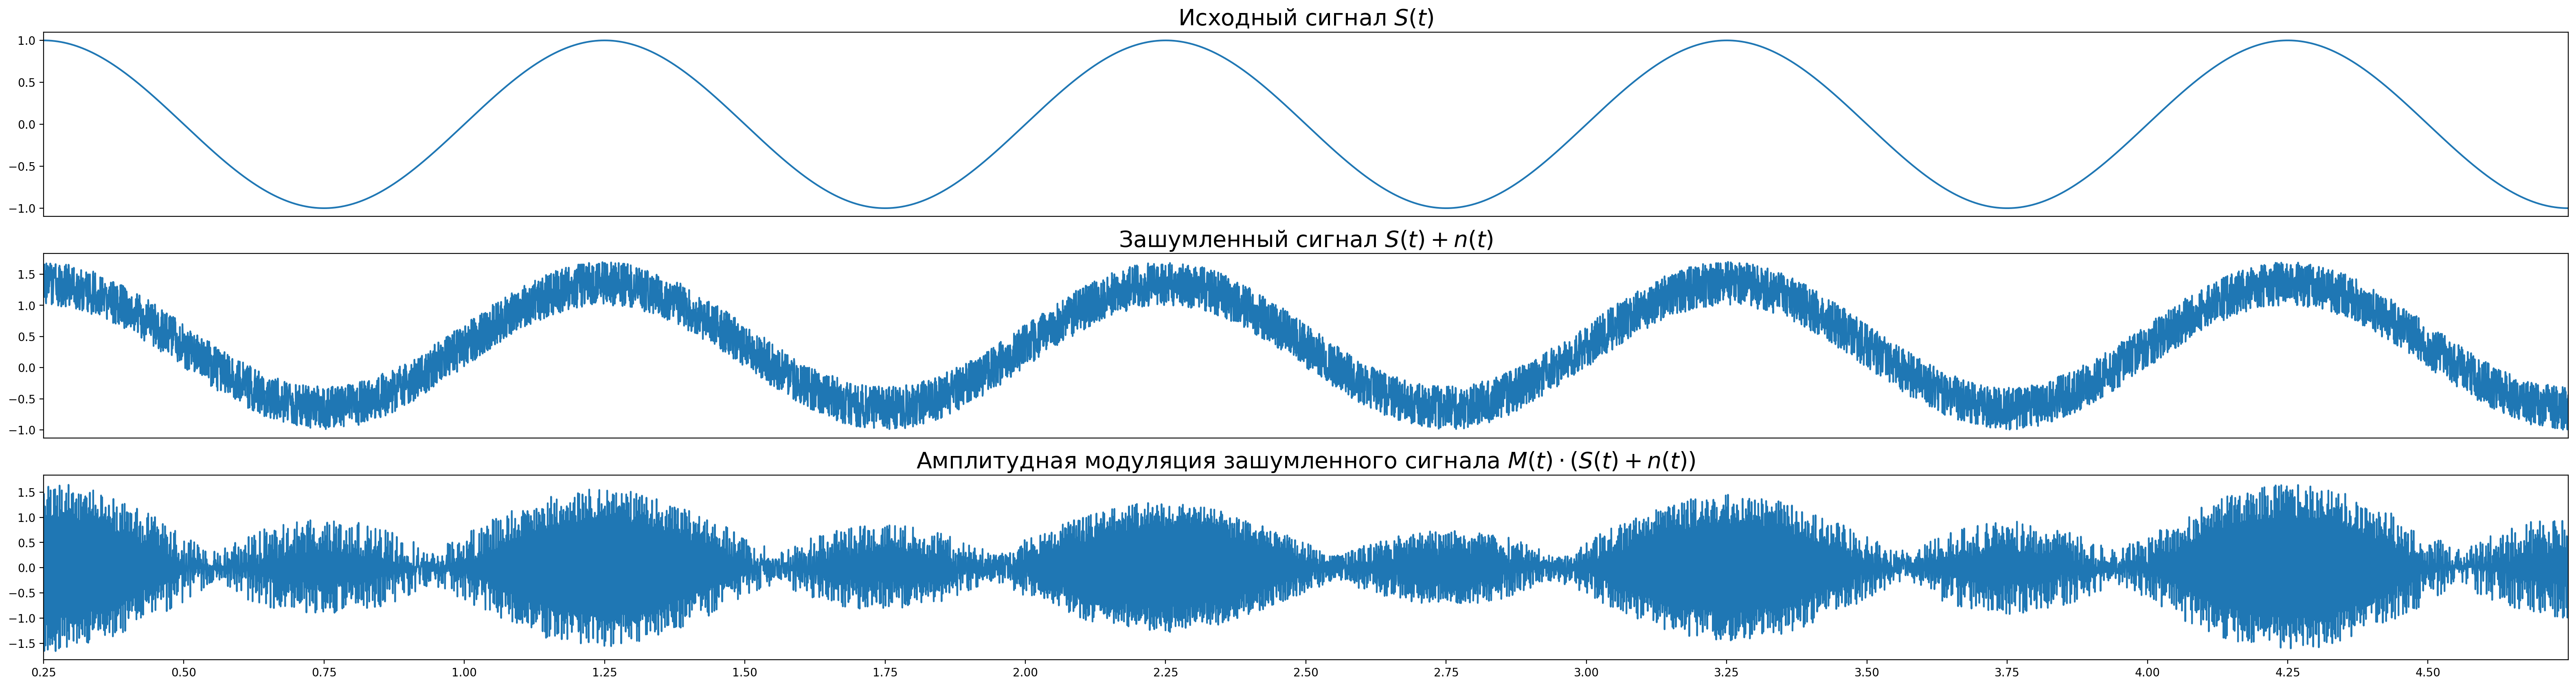
\includegraphics[width = 1 \textwidth]{input_signals.png}
    \caption{Полезный сигнал, зашумленный сигнал, амплитудная моуляция зашумленного сигнала}
    \label{fig:input_signals}
\end{figure}

Для увеличения динамического диапазона реализуем следующую схему:
\begin{enumerate}
    \item Подадим зашумленный сигнал на $bp$ фильтр, частота среза которого совпадает с частотой модулирующей синусоиды: $\hat{L}(M(t) \cdot [S(t) + n(t)])$
    \item Демодулируем отфильтрованный сигнал:  $\hat{L}(M(t) \cdot [S(t) + n(t)]) / M(t)$
\end{enumerate}

При помощи библиотеки $scipy.signal$ был проведен эксперимент по описанной методике. Результаты эксперимента представлены на рисунке \ref{fig:result_signal}, динамический диапазон был увеличен с $3 dB$ до $14 dB$.

\begin{figure}[htbp]
    \centering
    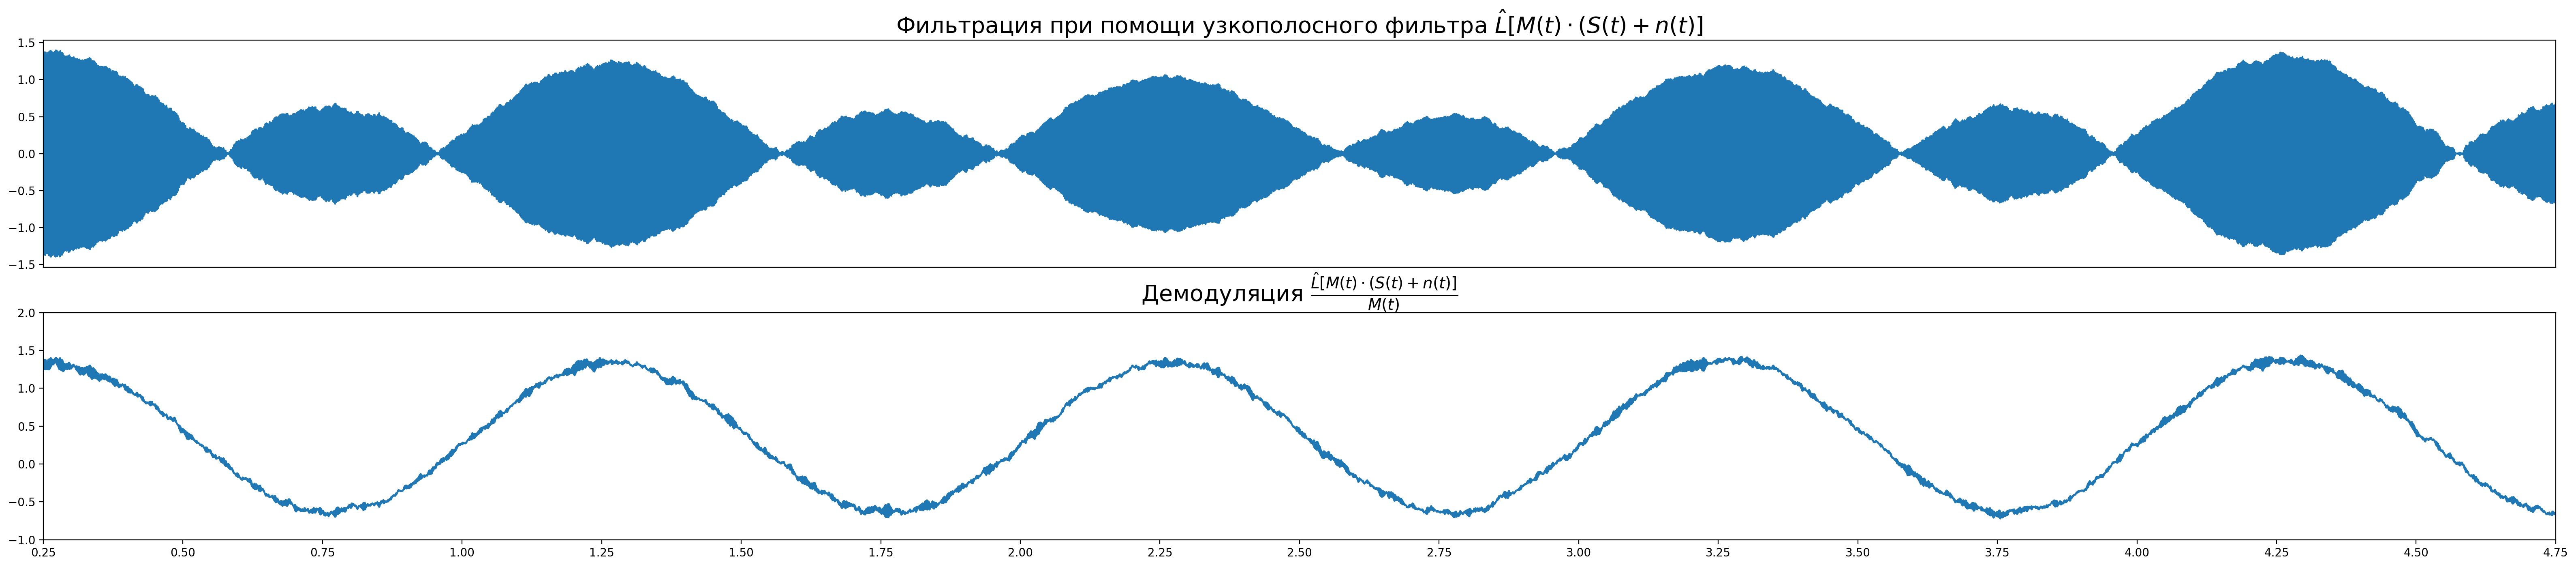
\includegraphics[width = \textwidth]{output_signals.png}
    \caption{Результат работы алгоритма}
    \label{fig:result_signal}
\end{figure}


\section*{\textcolor{header}{Обработка экспериментальных данных}}

Измерим зависимость амплитуды выходного сигнала от частоты колебаний динамика. Как видно на рисунке \ref{fig:freq}, наибольшая амплитуда достигается на часоте $\sim 26 \text{ Гц}$. Используем эту частоту для проведения дальнейших экспериментов.
\begin{figure}[htbp]
    \centering
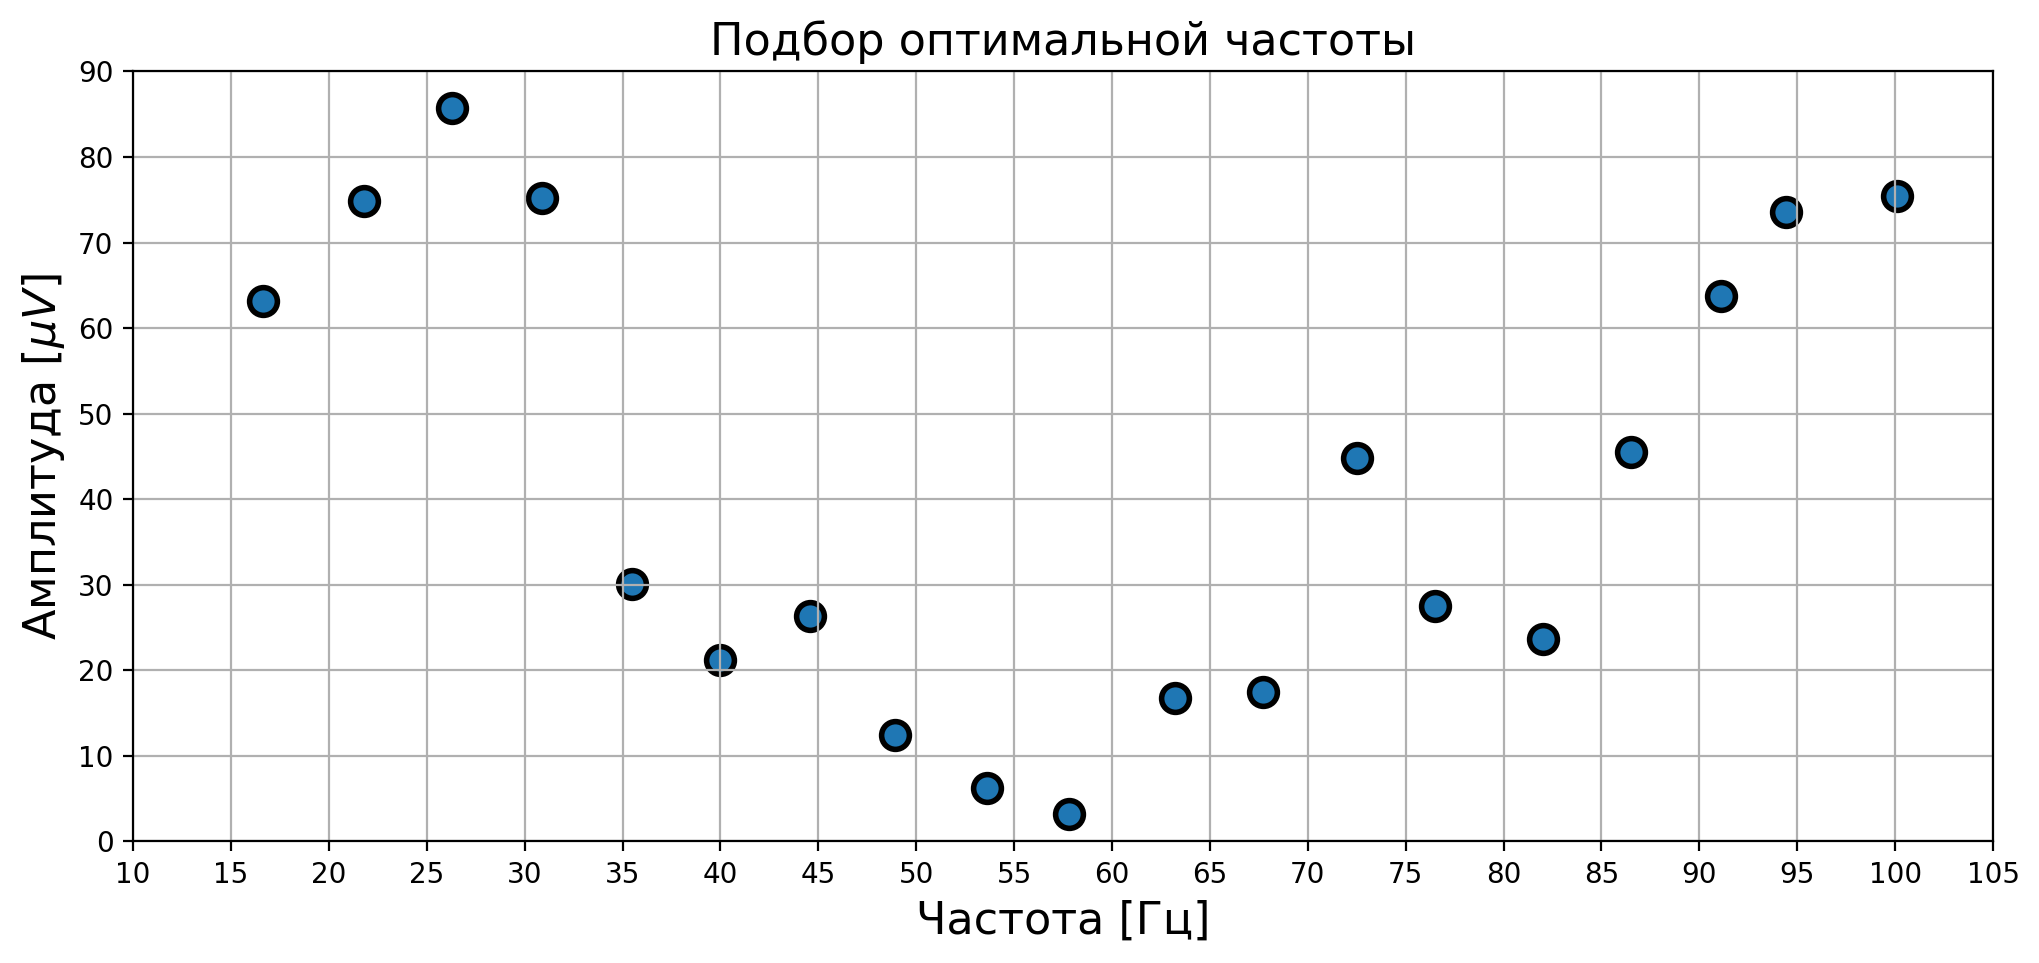
\includegraphics[width = 0.7 \textwidth]{freq.png}
    \caption{Результат эксперимента по подбору <<рабочей>> часоты}
    \label{fig:freq}
\end{figure}


Снимем зависимость амплитуды выходного сигнала от подаваемого на катушки напряжения.
\begin{figure}[htbp]
    \centering
    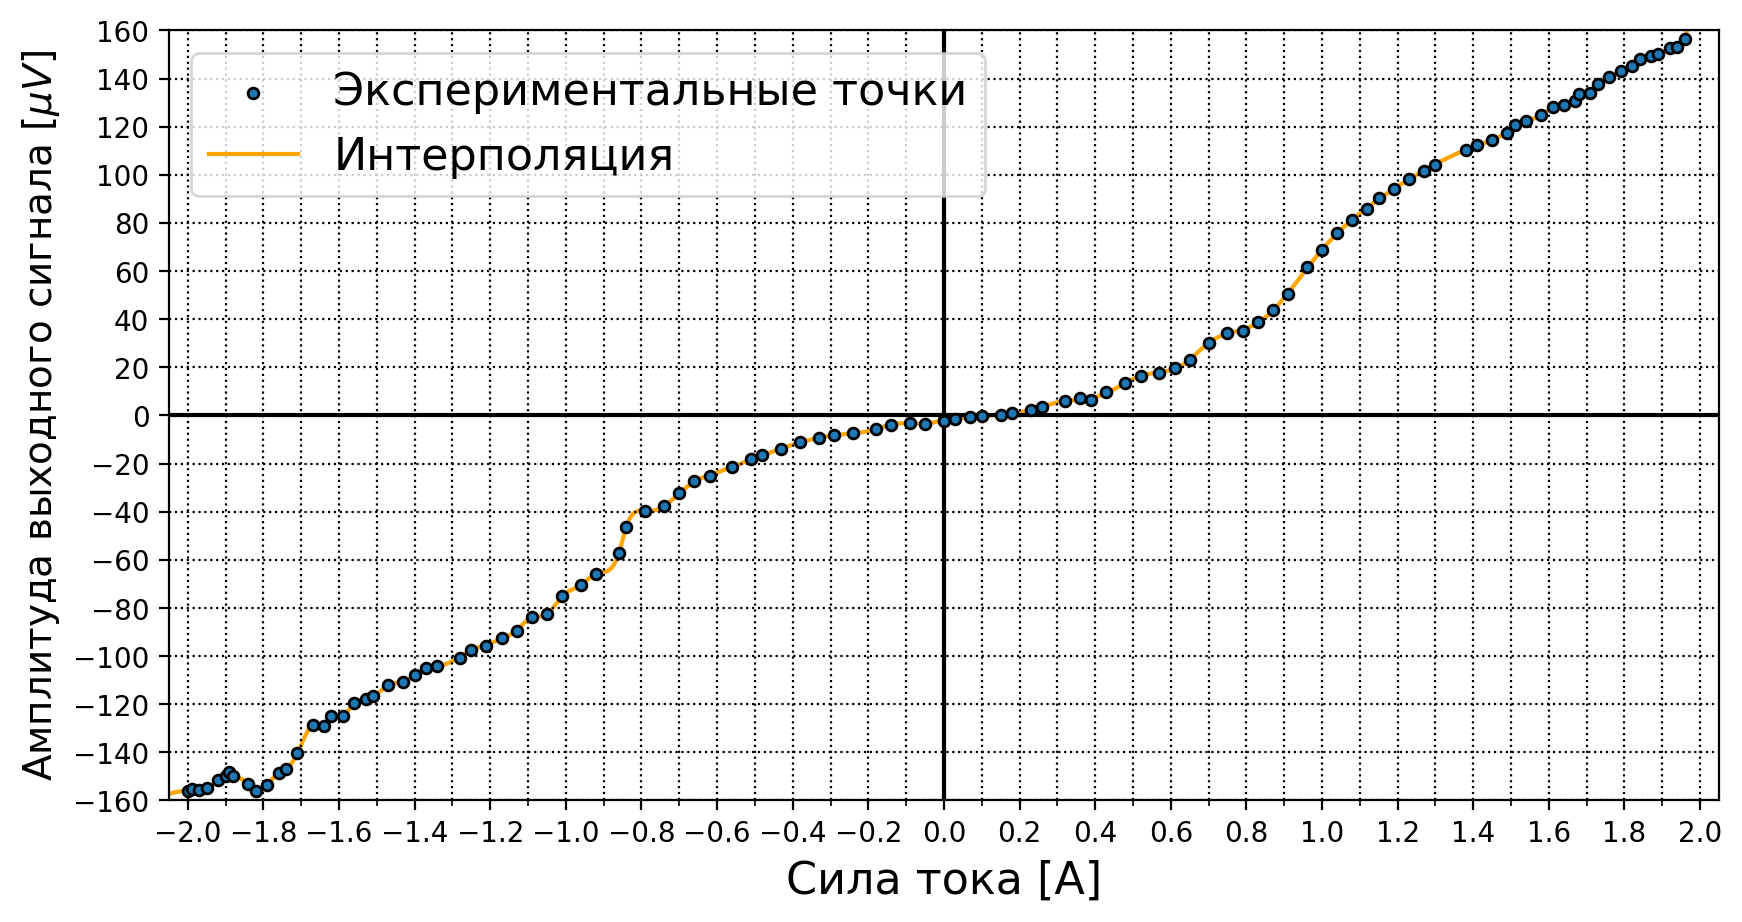
\includegraphics[width = 0.9 \textwidth]{magnetic_curve.png}
    \caption{Зависимость амплитуды выходного сигнала от силы тока, протекающего через катушки.}
    \label{fig:magnetic}
\end{figure}

График, представленный на рисунке \ref{fig:magnetic} по сути есть кривая намагничивания исследуемого образца. Поле, создаваемое катушками, пропорционально силе тока который через них протекает. Магнитный момент образца пропорционален амплитуде выходного сигнала.

\section*{\textcolor{header}{Вывод}}


Изучены основы конструирования и применения магнитометров с вибрирующим
образцом для определения магнитных параметров тонкой магнитной пленки. В процессе
работы мы получили зависимость ЭДС индукции от силы тока (поле в катушках) и
зависимость ЭДС индукции от частоты вибрации штока.



\end{document}
